\documentclass[12pt]{article}
\usepackage{fancyhdr, mathptmx, lastpage}
\usepackage{enumitem}
\usepackage{graphicx, caption, float}
\usepackage[a4paper, top=2.54cm, bottom=2.54cm, left=3.17cm, right=3.23cm]{geometry}

%%%%%%%%%%%%%%%%%%%%%%%%%%%%%
%%% SETUP CODE START HERE %%%
%%%%%%%%%%%%%%%%%%%%%%%%%%%%%

%% HEADER %%
% set the header and footer
\fancypagestyle{main}{
	\pagestyle{fancy}
	\addtolength{\headheight}{\baselineskip}
	%\renewcommand{\sectionmark}[1]{\markboth{#1}{}}
	%\renewcommand{\subsectionmark}[1]{\markright{#1}}
%	\rhead{\leftmark\\\rightmark}
	
	% set default header 
	\fancyhf{}
	\lhead{\textbf{SULIT}\\}
	\rhead{(\textbf{EN390})}
	\fancyhead[C]{\raisebox{-4ex}{-\thepage-}}
	\renewcommand{\headrulewidth}{0pt}
}

% set title page header 
\fancypagestyle{titlestyle}{
	\pagestyle{fancy}
	\fancyhf{}
	\lhead{\textbf{SULIT}}
	\renewcommand{\headrulewidth}{0pt}
}

% setting title page input
%% Semester
%\def\semester#1{\gdef\@semester{#1}}
%\def\@semester{\@latex@warning@no@line{No \noexpand\semester given}}
%
%%% Sidang
%\def\sidang#1{\gdef\@sidang{#1}}
%\def\@sidang{\@latex@warning@no@line{No \noexpand\sidang given}}
%
%%% Exam Month Year
%\def\examMonthYear#1{\gdef\@examMonthYear{#1}}
%\def\@examMonthYear{\@latex@warning@no@line{No \noexpand\examMonthYear given}}
%
%%% Course
%\def\courseCode#1{\gdef\@courseCode{#1}}
%\def\@courseCode{\@latex@warning@no@line{No \noexpand\courseCode given}}
%
%%% Course Name English
%\def\courseNameEn#1{\gdef\@courseNameEn{#1}}
%\def\@courseNameEn{\@latex@warning@no@line{No \noexpand\courseNameEn given}}
%
%%% Course Name Malay
%\def\courseNameBM#1{\gdef\@courseNameBM{#1}}
%\def\@courseNameBM{\@latex@warning@no@line{No \noexpand\courseNameBM given}}

%% FIGURE %%
% declare figure extension
\DeclareGraphicsExtensions{.png,.pdf}

% declare caption
\captionsetup[figure]{labelsep=newline, labelfont=bf}
\captionsetup[table]{labelsep=newline, labelfont=bf, position=top}



%% BODY TEXT %%
% set no paragraph indentation for the whole document
\setlength\parindent{0pt}

% setting the command question
\newcounter{counterquestion}
\newcommand{\question}{	 
	\stepcounter{counterquestion}{\textbf{QUESTION \thecounterquestion} \\
		\fontsize{10pt}{\baselineskip} \textbf{\emph{[SOALAN \thecounterquestion]}} \\
	}
}



% setting the command translation
\newcommand{\translation}[1]{
	\fontsize{10pt}{\baselineskip}
		\emph{#1}
}

% setting for marks
\newcommand{\qmarks}[1]{
	\mbox{}\hfill (#1 Marks/\fontsize{10pt}{\baselineskip}\emph{Markah})
}

%% ORDERED LIST %%
% define item label
\makeatletter
\def\namedlabel#1#2{\begingroup
	#2%
	\def\@currentlabel{#2}%
	\phantomsection\label{#1}\endgroup
}
\makeatother

% setup ordered list
%\renewcommand{\labelenumi}{(\alph{enumi})}
%\renewcommand{\labelenumii}{(\roman{enumii})}
%\renewcommand{\labelenumiii}{(\Alph{enumii})}
%\renewcommand{\labelenumiv}{(\Roman{enumii})}

% setup ordered list
\setlist[enumerate,1]{wide = 0pt, labelwidth = 1.5em, labelsep*=0em, leftmargin = \dimexpr\labelwidth + \labelsep\relax, label=(\alph*), ref=(\alph*)}
\setlist[enumerate,2]{wide = 0pt, labelwidth = 2em, labelsep*=0em, leftmargin = \dimexpr\labelwidth + \labelsep\relax, label=(\roman*), ref=(\roman*)}
\setlist[enumerate,3]{wide = 0pt, labelwidth = 2em, labelsep*=0em, leftmargin = \dimexpr\labelwidth + \labelsep\relax, label=(\Alph*), ref=(\Alph*)}
\setlist[enumerate,4]{wide = 0pt, labelwidth = 2em, labelsep*=0em, leftmargin = \dimexpr\labelwidth + \labelsep\relax, label=(\Roman*), ref=(\Roman*)}

% begin enumerate list, default spacing
\newcommand{\listbegin}{
	\begin{enumerate}%[leftmargin=0.65cm]
}	

% begin list, no spacing before the list
\newcommand{\listbeginx}{
	\begin{enumerate}[topsep=0pt]
}	
		
% close enumerate		
\newcommand{\listclose}{
	\end{enumerate}
}

%% PAGE NUMBER %%
% display next page
\newcommand{\nextpage}{%	
	\vfill \hfill 
	\ldots\the\numexpr\value{page}+1\relax/-
}

%%% SETUP TITLE PAGE %%%
%\semester{Kedua}
%\sidang{2017/2018}
%\examMonthYear{Jun 2018}
%\courseCode{ENT390}
%\courseNameEn{Bioinstrumentation 1}
%\courseNameBM{Bioinstrumentasi 1}

%%%%%%%%%%%%%%%%%%%%%%%%%%%
%%% SETUP CODE END HERE %%%
%%%%%%%%%%%%%%%%%%%%%%%%%%%

\begin{document}
% cover page

%\begin{titlepage}	
	\pagestyle{titlestyle}
	\vspace*{5\baselineskip}
	\hrule \vspace*{2\baselineskip}
%	\centering
	\begin{center}
		\textbf{UNIVERSITI MALAYSIA PERLIS}\\[\baselineskip]
		Peperiksaan Akhir Semester Kedua
\\
		Sidang Akademik 2017/2018
\\[2\baselineskip]
		Jun 2018 \\[\baselineskip]
		\textbf{ENT390 -- Bioinstrumentation 1 }\\
		\textbf{[Bioinstrumentasi 1]} \\[2\baselineskip]
		Masa: 3 jam \\[2\baselineskip]
		\hrule \vspace*{2\baselineskip}
	\end{center}
	
	Please make sure that this question paper has \textbf{SIX (\pageref{LastPage})} printed pages including this front page before you start the examination.
	
	\translation{%
		[Sila pastikan kertas soalan ini mengandungi \textbf{ENAM (\pageref{LastPage})} muka surat yang bercetak termasuk muka hadapan sebelum anda memulakan peperiksaan ini.]
	}\\

	This question paper has \textbf{TWO (2)} parts. Answer \textbf{all} questions in \mbox{\textbf{Part A}} and \mbox{\textbf{THREE (3)}} question in \mbox{\textbf{Part B}}. Each question contributes 25 marks. 
		
	\translation{%
		[Kertas soalan ini mengandungi \textbf{DUA (2)} bahagian. Jawab \textbf{semua} soalan di \mbox{\textbf{Bahagian A}} dan \mbox{\textbf{TIGA (3)}} soalan di \mbox{\textbf{Bahagian B}}. Setiap soalan menyumbang 25 markah.]
	}
	
	\clearpage
	
%\end{titlepage}

\pagestyle{main}
\vspace*{1mm}
\setcounter{page}{2}

%%%%%%%%%%%%%%%%%%%%%%%%%%%%
%%% MAIN BODY START HERE %%%
%%%%%%%%%%%%%%%%%%%%%%%%%%%%


% setting newpart counter
\newcounter{counterpart}
\newcommand{\newpart}{	 	
	\stepcounter{counterpart}
	\setcounter{counterquestion}{0}
	\textbf{\Alph{counterpart}}
}

% setting the command question. used together with \newpart
\newcommand{\partQuestion}{	 
	\stepcounter{counterquestion}{\textbf{QUESTION \Alph{counterpart}\thecounterquestion} \\
		\fontsize{10pt}{\baselineskip} \textbf{\emph{[SOALAN \Alph{counterpart}\thecounterquestion]}} \\
	}
}

% PART A
\textbf{Part \newpart: Answer all questions} \\
\textbf{\translation{[Bahagian \Alph{counterpart}: Jawab semua soalan]}}
\\

\partQuestion
%% Question 1
\question

\listbeginx	% start 1st level question
	\item \label{chemical} What chemical reactions you expect to see at these electrodes? 
	
	\translation{Apakah tindak balas kimia yang anda jangka dapat dilihat pada kedua –dua elektrod} 
	
	\qmarks{4}	% define marks
	
	\item A pair of biopotential electrodes is implanted in an animal to measure the electrocardiogram.
	
	\translation{Sepasang elektrod biopotensi diimplan ke dalam haiwan untuk mengukur elektrokardiogram.}

	\listbegin	% start 2nd level question
		\item Based on \ref{chemical}, explain what will happen if the electrodes were shorted together. Explain what will happen if the electrodes were shorted together. 
		
		\translation{Terangkan apakah yang akan berlaku apabila kedua – kedua elektrod disambung?. Terangkan apakah yang akan berlaku apabila kedua – kedua elektrod disambung?} 
		
		\qmarks{2} % define marks
	\listclose % close 2nd level question
	
	\item Explain what will happen if the capacitor in \cref{fig:meshcircuit} were shorted. 
	
	\translation{Terangkan apakah yang akan berlaku apabila kedua – kedua elektrod disambung?} 
	
	\qmarks{3} % define marks
		
	\begin{figure}[H] % H means, to put figure here after the code
		\centering
%		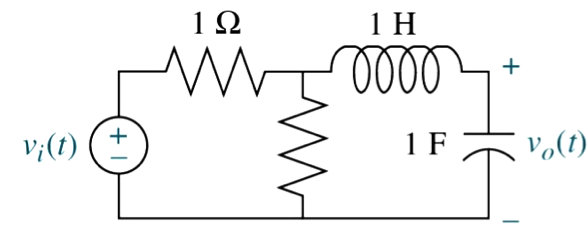
\includegraphics[width=0.5\textwidth]{testfig}
		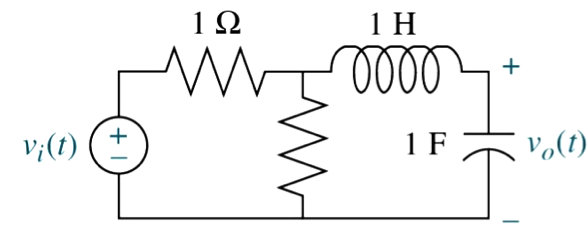
\includegraphics{testfig}
		\caption{\rajah}
		\label{fig:meshcircuit}
	\end{figure}

	% Table generated by Excel2LaTeX from sheet 'Sheet1'
	\begin{table}[H]
		\centering
		\caption{\jadual}
		\begin{tabular}{cc}
			\toprule
			\multicolumn{1}{l}{\textbf{Frequency}} & \multicolumn{1}{l}{\textbf{Impedance (Magnitude) ($\Omega$)}} \\
			\midrule
			5 Hz  & 20,000 \\
			10 Hz & 19,998 \\
			\vdots     & \vdots \\
			40 kHz & 602 \\
			50 kHz & 600 \\
			100 kHz & 600 \\
			\bottomrule
		\end{tabular}%
		\label{table:freqmag}%
	\end{table}%
\listclose % close 1st level question



% PART B
\textbf{Part \newpart: Answer any THREE (3) questions } \\
\textbf{\translation{[Bahagian \Alph{counterpart}: Jawab mana-mana TIGA (3) soalan]}}
\\

\partQuestion
%% Question 2
\question

% question without enumerate list
Silver/silver chloride (Ag/AgCl) electrodes are commonly used in biological measurement.

\translation{Elektrod Argentum/Argentum chloride (Ag/AgCl) digunakan secara meluas didalam pengukuran biologi}	

\qmarks{5}

\listbegin	% start 1st level question
	\item \label{halfmembrane} State the definition of half-membrane
	
	\translation{Nyatakan definisi separuh-membran}
	
	\qmarks{2}
	
	\item \label{itm:net} Elaborate the basic mechanisms that contribute to condition in \ref{halfmembrane}, and write its net potential. % use label to reference to the list item
	
	\translation{Kembangkan mekanisma asas yang menyumbang kepada keadaan di \ref{halfmembrane}, dan tuliskan upaya bersih.}
	
	\qmarks{4}

	\listbegin % start 2nd level question
		\item \label{itm:ref2nd} Second level item that refer to \ref{itm:net}. Second level item. second level item. 
		
		\translation{ini adalah level kedua. ini adalah level kedua. ini adalah level kedua.} 
		
		\item Another second level that refer to \ref{itm:ref2nd}. Another second level. Another second level.
		
		\translation{ini adalah level kedua. ini adalah level kedua. ini adalah level kedua.} 
		
		\item Another second level that refer to \ref{itm:ref2nd}. Another second level. Another second level.
		
		\translation{ini adalah level kedua. ini adalah level kedua. ini adalah level kedua.} 
		
		\item Another second level that refer to \ref{itm:ref2nd}. Another second level. Another second level.
		
		\translation{ini adalah level kedua. ini adalah level kedua. ini adalah level kedua.} 


		\listbegin % start 3rd level question
			\item Another level. This is third level. This is third level. This is third level. This is third level
			
			\translation{Ini adalah level ketiga. Ini adalah level ketiga. Ini adalah level ketiga. Ini adalah level ketiga. Ini adalah level ketiga. Ini adalah level ketiga}

			\listbegin  % start 4th level question
				\item Another level. This is fourth level. This is fourth level. This is fourth level. This is fourth level. 
				
				\translation{Ini adalah level keempat. Ini adalah level keempat. Ini adalah level keempat. Ini adalah level keempat.}
			\listclose % close 4th level question
		\listclose % close 3rd level question
	\listclose % close 2nd level question
\listclose	% close 1st level question
%% Question 3
\clearpage	% start new page
\question

Some questions here...


%% Question 4
\clearpage	% start new page
\question

Silver/silver chloride (Ag/AgCl) electrodes are commonly used in biological measurement. 

\translation{Elektrod Argentum/Argentum chloride (Ag/AgCl) digunakan secara meluas didalam pengukuran biologi}	

\listbegin	% start 1st level question
	\item \label{halfmembrane} State the definition of half-membrane
	
	\translation{some translation here}
	
	\qmarks{2}
	
	\answer{Put answer to this question here. This answer scheme can be turned on and off by executing \texttt{answers} option. Refer to manual for explanation.
	} 
	
	\item \label{itm:net} Elaborate the basic mechanisms that contribute to condition in \ref{halfmembrane}, and write its net potential. % use label to reference to the list item
	
	\translation{some translation here}
	
	\qmarks{2}
	
	\answer{Put answer to this question here. This answer scheme can be turned on and off by executing \texttt{answers} option. Refer to manual for explanation.
	} 

	\listbegin % start 2nd level question
		\item \label{itm:ref2nd} Second level item that refer to \ref{itm:net}. Second level item. second level item. \\
		\translation{ini adalah level kedua. ini adalah level kedua. ini adalah level kedua.} 
		
		\qmarks{3}
		
		\answer{Put answer to this question here. This answer scheme can be turned on and off by executing \texttt{answers} option. Refer to manual for explanation.
		} 

		\listbegin % start 3rd level question
			\item Another level. This is third level. This is third level. This is third level. This is third level\\
			\translation{Ini adalah level ketiga. Ini adalah level ketiga. Ini adalah level ketiga. Ini adalah level ketiga. Ini adalah level ketiga. Ini adalah level ketiga.}
		\listclose % close 3rd level question
	\listclose	% close 2nd level question	
\listclose	% close 1st level question	

%% Question 5
\clearpage	% start new page
\question

	\answer{ 
		This is the answer to the question 5. This answer scheme can be turned on and off by executing \texttt{answers} option. Refer to manual for explanation.
	}




\vskip 20ex\centering\bfseries -oooOooo-	

\end{document}